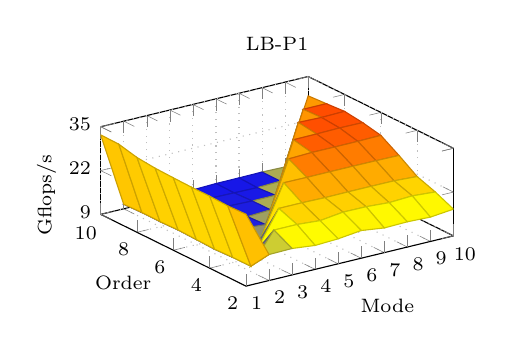
\begin{tikzpicture}
\begin{axis}[height=0.35\textwidth,width=0.5\textwidth,style={font=\scriptsize},grid=major,grid style={dotted},align=center,xlabel={Mode}, ylabel={Order},zlabel={Gflops/s},title={\ttt{LB-P1}}, xtick={1,2,3,4,5,6,7,8,9,10},xticklabels={1,2,3,4,5,6,7,8,9,10}, ytick={2,4,6,8,10}, yticklabels={2,4,6,8,10}, point meta max=35, point meta min=9, zmin=9, zmax=35, ztick={9,22,35}, zticklabels={9,22,35}, view={-35}{45}, xlabel style={yshift=2mm}, ylabel style={yshift=4mm}, zlabel style={yshift=-1mm,xshift=-4mm}]
\addplot3[surf] %, colormap = {whiteblack}{color(0cm)=(white);color(0.4cm) = (darkgray)}
coordinates{
(1.000,2.000,30.340) (1.000,3.000,30.150) (1.000,4.000,30.377) (1.000,5.000,30.377) (1.000,6.000,30.496) (1.000,7.000,30.686) (1.000,8.000,31.196) (1.000,9.000,32.484) (1.000,10.000,32.591) 
	
(2.000,2.000,16.722) (2.000,3.000,10.585) (2.000,4.000,10.550) (2.000,5.000,10.314) (2.000,6.000,10.511) (2.000,7.000,10.673) (2.000,8.000,10.503) (2.000,9.000,10.548) (2.000,10.000,10.332) 

(3.000,2.000,16.857) (3.000,3.000,19.659) (3.000,4.000,10.526) (3.000,5.000,10.205) (3.000,6.000,10.288) (3.000,7.000,10.147) (3.000,8.000,10.260) (3.000,9.000,9.797) (3.000,10.000,10.055) 

(4.000,2.000,16.102) (4.000,3.000,19.651) (4.000,4.000,21.764) (4.000,5.000,10.137) (4.000,6.000,10.555) (4.000,7.000,10.015) (4.000,8.000,10.299) (4.000,9.000,10.105) (4.000,10.000,9.908) 

(5.000,2.000,16.414) (5.000,3.000,19.135) (5.000,4.000,21.771) (5.000,5.000,25.061) (5.000,6.000,9.984) (5.000,7.000,9.693) (5.000,8.000,10.201) (5.000,9.000,9.856) (5.000,10.000,9.636) 

(6.000,2.000,17.213) (6.000,3.000,20.011) (6.000,4.000,21.633) (6.000,5.000,24.989) (6.000,6.000,27.821) (6.000,7.000,10.053) (6.000,8.000,10.014) (6.000,9.000,9.749) (6.000,10.000,9.862) 

(7.000,2.000,16.320) (7.000,3.000,19.956) (7.000,4.000,21.696) (7.000,5.000,25.002) (7.000,6.000,28.062) (7.000,7.000,29.186) (7.000,8.000,10.048) (7.000,9.000,9.639) (7.000,10.000,9.882) 
	
(8.000,2.000,16.492) (8.000,3.000,19.515) (8.000,4.000,21.696) (8.000,5.000,25.000) (8.000,6.000,28.036) (8.000,7.000,29.241) (8.000,8.000,30.006) (8.000,9.000,9.911) (8.000,10.000,9.964) 
	
(9.000,2.000,16.228) (9.000,3.000,19.860) (9.000,4.000,21.672) (9.000,5.000,24.976) (9.000,6.000,28.062) (9.000,7.000,29.371) (9.000,8.000,29.826) (9.000,9.000,29.590) (9.000,10.000,9.821) 
	
(10.000,2.000,16.926) (10.000,3.000,19.364) (10.000,4.000,21.283) (10.000,5.000,24.884) (10.000,6.000,28.180) (10.000,7.000,29.297) (10.000,8.000,29.988) (10.000,9.000,29.598) (10.000,10.000,29.257) 
	
};\end{axis}
\end{tikzpicture}
\begin{comment}
\begin{tikzpicture}
\begin{axis}[height=0.40\textheight,width=0.40\textwidth,style={font=\footnotesize},grid=major,grid style={dotted},align=center,xlabel={Kontraktionsmodus},ylabel={Tensorstufe},title={{LB}-{P1}},scaled ticks=false,zticklabel=\pgfmathprintnumber{\tick},zlabel={Durchsatz [Gflops/s]},view={-45}{45}, zlabel={Standardfehler [\%]}]
\addplot3[surf]
coordinates{(1.000,2.000,1.865) (1.000,3.000,2.919) (1.000,4.000,3.127) (1.000,5.000,3.522) (1.000,6.000,4.168) (1.000,7.000,4.511) (1.000,8.000,4.143) (1.000,9.000,1.151) (1.000,10.000,1.071) 
	
	(2.000,2.000,1.262) (2.000,3.000,9.168) (2.000,4.000,12.462) (2.000,5.000,10.166) (2.000,6.000,11.619) (2.000,7.000,11.462) (2.000,8.000,10.765) (2.000,9.000,11.361) (2.000,10.000,11.626) 
	
	(3.000,2.000,4.592) (3.000,3.000,1.071) (3.000,4.000,8.620) (3.000,5.000,11.768) (3.000,6.000,8.149) (3.000,7.000,11.048) (3.000,8.000,12.646) (3.000,9.000,10.426) (3.000,10.000,11.319) 
	
	(4.000,2.000,2.505) (4.000,3.000,0.801) (4.000,4.000,1.578) (4.000,5.000,11.887) (4.000,6.000,12.483) (4.000,7.000,10.515) (4.000,8.000,8.651) (4.000,9.000,12.485) (4.000,10.000,12.117) 
	
	(5.000,2.000,3.123) (5.000,3.000,1.145) (5.000,4.000,1.532) (5.000,5.000,2.987) (5.000,6.000,11.781) (5.000,7.000,11.819) (5.000,8.000,9.498) (5.000,9.000,11.849) (5.000,10.000,11.091) 
	
	(6.000,2.000,3.540) (6.000,3.000,1.277) (6.000,4.000,1.801) (6.000,5.000,2.805) (6.000,6.000,2.525) (6.000,7.000,8.015) (6.000,8.000,13.387) (6.000,9.000,8.782) (6.000,10.000,10.696) 
	
	(7.000,2.000,3.614) (7.000,3.000,1.138) (7.000,4.000,1.704) (7.000,5.000,2.909) (7.000,6.000,2.451) (7.000,7.000,1.946) (7.000,8.000,11.372) (7.000,9.000,11.030) (7.000,10.000,12.054) 
	
	(8.000,2.000,4.086) (8.000,3.000,1.392) (8.000,4.000,1.646) (8.000,5.000,3.144) (8.000,6.000,2.326) (8.000,7.000,1.922) (8.000,8.000,1.426) (8.000,9.000,10.847) (8.000,10.000,9.075) 
	
	(9.000,2.000,3.670) (9.000,3.000,1.277) (9.000,4.000,1.418) (9.000,5.000,2.937) (9.000,6.000,2.300) (9.000,7.000,1.882) (9.000,8.000,1.527) (9.000,9.000,0.967) (9.000,10.000,10.730) 
	
	(10.000,2.000,3.497) (10.000,3.000,1.058) (10.000,4.000,1.789) (10.000,5.000,3.050) (10.000,6.000,2.069) (10.000,7.000,1.794) (10.000,8.000,1.428) (10.000,9.000,0.969) (10.000,10.000,0.529) 
	
};\end{axis}
\end{tikzpicture}
\end{comment}
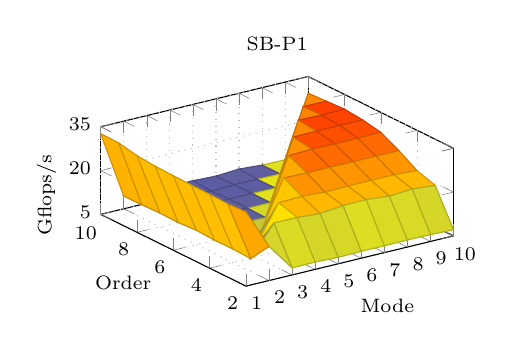
\begin{tikzpicture}
\begin{axis}[height=0.35\textwidth,width=0.5\textwidth,style={font=\scriptsize},grid=major,grid style={dotted},align=center,xlabel={Mode},ylabel={Order},zlabel={Gflops/s},title={\ttt{SB-P1}}, xtick={1,2,3,4,5,6,7,8,9,10},xticklabels={1,2,3,4,5,6,7,8,9,10}, ytick={2,4,6,8,10}, yticklabels={2,4,6,8,10}, point meta max=35, point meta min=5, zmin=5, zmax=35, ztick={5,20,35}, zticklabels={5,20,35}, view={-35}{45}, xlabel style={yshift=2mm}, ylabel style={yshift=4mm}, zlabel style={yshift=-1mm,xshift=-4mm}]
\addplot3[surf] % , colormap = {whiteblack}{color(0cm)=(white);color(0.4cm) = (darkgray)}
coordinates{
(1.000,2.000,30.432) (1.000,3.000,30.105) (1.000,4.000,30.292) (1.000,5.000,30.361) (1.000,6.000,30.537) (1.000,7.000,30.721) (1.000,8.000,31.253) (1.000,9.000,32.509) (1.000,10.000,32.643) 

(2.000,2.000,16.708) (2.000,3.000,9.472) (2.000,4.000,9.724) (2.000,5.000,9.652) (2.000,6.000,9.963) (2.000,7.000,9.546) (2.000,8.000,9.694) (2.000,9.000,9.463) (2.000,10.000,9.405) 

(3.000,2.000,7.397) (3.000,3.000,19.720) (3.000,4.000,8.618) (3.000,5.000,9.043) (3.000,6.000,9.168) (3.000,7.000,9.161) (3.000,8.000,8.551) (3.000,9.000,8.307) (3.000,10.000,8.404) 

(4.000,2.000,7.495) (4.000,3.000,19.656) (4.000,4.000,21.706) (4.000,5.000,8.562) (4.000,6.000,8.778) (4.000,7.000,8.882) (4.000,8.000,8.704) (4.000,9.000,8.760) (4.000,10.000,8.724) 

(5.000,2.000,7.187) (5.000,3.000,19.134) (5.000,4.000,21.919) (5.000,5.000,25.134) (5.000,6.000,8.534) (5.000,7.000,8.679) (5.000,8.000,8.767) (5.000,9.000,8.350) (5.000,10.000,8.891) 

(6.000,2.000,7.370) (6.000,3.000,19.899) (6.000,4.000,21.481) (6.000,5.000,24.987) (6.000,6.000,27.823) (6.000,7.000,8.658) (6.000,8.000,8.711) (6.000,9.000,8.624) (6.000,10.000,8.539) 

(7.000,2.000,7.310) (7.000,3.000,20.082) (7.000,4.000,21.602) (7.000,5.000,24.982) (7.000,6.000,28.118) (7.000,7.000,29.190) (7.000,8.000,8.681) (7.000,9.000,8.601) (7.000,10.000,9.051) 

(8.000,2.000,7.424) (8.000,3.000,19.351) (8.000,4.000,21.686) (8.000,5.000,24.979) (8.000,6.000,28.026) (8.000,7.000,29.333) (8.000,8.000,30.003) (8.000,9.000,8.518) (8.000,10.000,8.490) 

(9.000,2.000,7.317) (9.000,3.000,19.880) (9.000,4.000,21.646) (9.000,5.000,24.979) (9.000,6.000,28.078) (9.000,7.000,29.364) (9.000,8.000,29.802) (9.000,9.000,29.655) (9.000,10.000,8.382) 

(10.000,2.000,7.117) (10.000,3.000,19.176) (10.000,4.000,21.198) (10.000,5.000,24.958) (10.000,6.000,28.156) (10.000,7.000,29.342) (10.000,8.000,29.950) (10.000,9.000,29.630) (10.000,10.000,29.294) 

};
\end{axis}
\end{tikzpicture}
\begin{comment}
\begin{tikzpicture}
\begin{axis}[height=0.40\textheight,width=0.40\textwidth,style={font=\footnotesize},grid=major,grid style={dotted},align=center,xlabel={Kontraktionsmodus},ylabel={Tensorstufe},title={TLib-SB-{P1}},scaled ticks=false,zticklabel=\pgfmathprintnumber{\tick},zlabel={Durchsatz [Gflops/s]},view={-45}{45}, zlabel={Standardfehler [\%]}]
\addplot3[surf]
coordinates{(1.000,2.000,2.166) (1.000,3.000,2.892) (1.000,4.000,3.520) (1.000,5.000,3.679) (1.000,6.000,4.069) (1.000,7.000,4.572) (1.000,8.000,4.220) (1.000,9.000,1.113) (1.000,10.000,0.757) 

(2.000,2.000,1.392) (2.000,3.000,12.181) (2.000,4.000,11.639) (2.000,5.000,12.297) (2.000,6.000,13.483) (2.000,7.000,11.327) (2.000,8.000,11.608) (2.000,9.000,10.021) (2.000,10.000,7.762) 

(3.000,2.000,0.605) (3.000,3.000,0.922) (3.000,4.000,7.262) (3.000,5.000,11.507) (3.000,6.000,10.980) (3.000,7.000,13.088) (3.000,8.000,10.499) (3.000,9.000,7.891) (3.000,10.000,10.541) 

(4.000,2.000,1.318) (4.000,3.000,0.895) (4.000,4.000,1.614) (4.000,5.000,11.723) (4.000,6.000,10.371) (4.000,7.000,10.552) (4.000,8.000,10.448) (4.000,9.000,11.639) (4.000,10.000,9.715) 

(5.000,2.000,0.444) (5.000,3.000,1.269) (5.000,4.000,1.329) (5.000,5.000,2.894) (5.000,6.000,12.131) (5.000,7.000,9.577) (5.000,8.000,12.183) (5.000,9.000,10.336) (5.000,10.000,9.377) 

(6.000,2.000,0.484) (6.000,3.000,1.237) (6.000,4.000,2.109) (6.000,5.000,2.884) (6.000,6.000,2.497) (6.000,7.000,11.915) (6.000,8.000,10.138) (6.000,9.000,10.479) (6.000,10.000,7.941) 

(7.000,2.000,0.432) (7.000,3.000,0.895) (7.000,4.000,1.727) (7.000,5.000,3.155) (7.000,6.000,2.530) (7.000,7.000,2.054) (7.000,8.000,9.984) (7.000,9.000,9.380) (7.000,10.000,9.855) 

(8.000,2.000,0.914) (8.000,3.000,1.192) (8.000,4.000,1.724) (8.000,5.000,3.100) (8.000,6.000,2.479) (8.000,7.000,1.911) (8.000,8.000,1.571) (8.000,9.000,8.906) (8.000,10.000,9.600) 

(9.000,2.000,0.373) (9.000,3.000,1.424) (9.000,4.000,1.392) (9.000,5.000,2.961) (9.000,6.000,2.325) (9.000,7.000,1.999) (9.000,8.000,1.713) (9.000,9.000,1.236) (9.000,10.000,8.944) 

(10.000,2.000,0.397) (10.000,3.000,1.321) (10.000,4.000,1.594) (10.000,5.000,3.096) (10.000,6.000,2.287) (10.000,7.000,1.961) (10.000,8.000,1.488) (10.000,9.000,0.959) (10.000,10.000,0.535) 

};\end{axis}
\end{tikzpicture}
\end{comment}

%%%%%%%%%%%%%%%%%%%%%%%%%%%

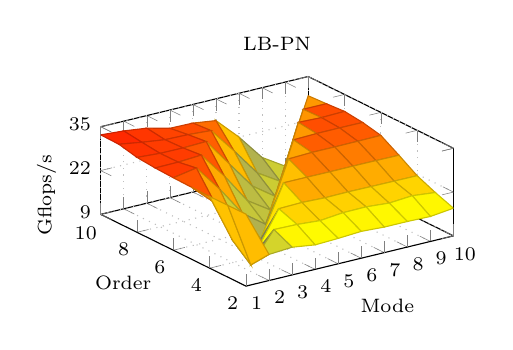
\begin{tikzpicture}
\begin{axis}[height=0.35\textwidth,width=0.5\textwidth,style={font=\scriptsize},grid=major,grid style={dotted},align=center,xlabel={Mode},ylabel={Order},zlabel={Gflops/s},title={\ttt{LB-PN}}, xtick={1,2,3,4,5,6,7,8,9,10},xticklabels={1,2,3,4,5,6,7,8,9,10}, ytick={2,4,6,8,10}, yticklabels={2,4,6,8,10}, point meta max=35, point meta min=9, zmin=9, zmax=35, ztick={9,22,35}, zticklabels={9,22,35}, view={-35}{45}, xlabel style={yshift=2mm}, ylabel style={yshift=4mm}, zlabel style={yshift=-1mm,xshift=-4mm}]
\addplot3[surf] %, colormap = {whiteblack}{color(0cm)=(white);color(0.4cm) = (darkgray)}
coordinates{
(1.000,2.000,30.353) (1.000,3.000,30.312) (1.000,4.000,30.265) (1.000,5.000,30.361) (1.000,6.000,30.506) (1.000,7.000,30.751) (1.000,8.000,31.224) (1.000,9.000,32.470) (1.000,10.000,32.590) 

(2.000,2.000,16.748) (2.000,3.000,10.971) (2.000,4.000,15.539) (2.000,5.000,24.166) (2.000,6.000,31.744) (2.000,7.000,30.820) (2.000,8.000,30.771) (2.000,9.000,31.394) (2.000,10.000,32.110) 

(3.000,2.000,17.232) (3.000,3.000,19.809) (3.000,4.000,10.343) (3.000,5.000,15.135) (3.000,6.000,23.893) (3.000,7.000,31.252) (3.000,8.000,30.718) (3.000,9.000,30.505) (3.000,10.000,31.268) 

(4.000,2.000,16.270) (4.000,3.000,19.656) (4.000,4.000,21.676) (4.000,5.000,9.964) (4.000,6.000,14.975) (4.000,7.000,23.383) (4.000,8.000,30.969) (4.000,9.000,30.341) (4.000,10.000,29.576) 

(5.000,2.000,16.531) (5.000,3.000,19.141) (5.000,4.000,21.867) (5.000,5.000,25.058) (5.000,6.000,10.071) (5.000,7.000,14.425) (5.000,8.000,22.690) (5.000,9.000,29.897) (5.000,10.000,29.463) 

(6.000,2.000,16.960) (6.000,3.000,19.837) (6.000,4.000,21.600) (6.000,5.000,25.039) (6.000,6.000,27.817) (6.000,7.000,9.995) (6.000,8.000,14.451) (6.000,9.000,22.192) (6.000,10.000,28.544) 

(7.000,2.000,16.580) (7.000,3.000,19.918) (7.000,4.000,21.691) (7.000,5.000,24.989) (7.000,6.000,28.077) (7.000,7.000,29.165) (7.000,8.000,9.692) (7.000,9.000,14.040) (7.000,10.000,21.983) 

(8.000,2.000,16.580) (8.000,3.000,19.375) (8.000,4.000,21.619) (8.000,5.000,25.026) (8.000,6.000,28.052) (8.000,7.000,29.365) (8.000,8.000,30.029) (8.000,9.000,9.851) (8.000,10.000,14.291) 

(9.000,2.000,16.414) (9.000,3.000,19.905) (9.000,4.000,21.575) (9.000,5.000,25.011) (9.000,6.000,28.093) (9.000,7.000,29.394) (9.000,8.000,29.785) (9.000,9.000,29.598) (9.000,10.000,10.064) 

(10.000,2.000,17.212) (10.000,3.000,19.196) (10.000,4.000,21.529) (10.000,5.000,24.939) (10.000,6.000,28.175) (10.000,7.000,29.346) (10.000,8.000,29.977) (10.000,9.000,29.587) (10.000,10.000,29.286) 

};
\end{axis}
\end{tikzpicture}
\begin{comment}
\begin{tikzpicture}
\begin{axis}[height=0.40\textheight,width=0.40\textwidth,style={font=\footnotesize},grid=major,grid style={dotted},align=center,xlabel={Kontraktionsmodus},ylabel={Tensorstufe},title={TLib-{LB}-{P2}},scaled ticks=false,zticklabel=\pgfmathprintnumber{\tick},zlabel={Durchsatz [Gflops/s]},view={-45}{45}, zlabel={Standardfehler [\%]}]
\addplot3[surf]
coordinates{(1.000,2.000,1.898) (1.000,3.000,2.533) (1.000,4.000,3.595) (1.000,5.000,3.637) (1.000,6.000,4.113) (1.000,7.000,4.502) (1.000,8.000,4.207) (1.000,9.000,1.266) (1.000,10.000,0.884) 

(2.000,2.000,1.169) (2.000,3.000,11.043) (2.000,4.000,6.645) (2.000,5.000,2.391) (2.000,6.000,1.025) (2.000,7.000,4.511) (2.000,8.000,1.619) (2.000,9.000,0.693) (2.000,10.000,0.822) 

(3.000,2.000,1.320) (3.000,3.000,0.851) (3.000,4.000,9.683) (3.000,5.000,5.843) (3.000,6.000,3.221) (3.000,7.000,1.216) (3.000,8.000,0.984) (3.000,9.000,1.380) (3.000,10.000,1.076) 

(4.000,2.000,1.325) (4.000,3.000,0.745) (4.000,4.000,1.694) (4.000,5.000,11.366) (4.000,6.000,6.330) (4.000,7.000,3.547) (4.000,8.000,0.999) (4.000,9.000,1.225) (4.000,10.000,1.703) 

(5.000,2.000,1.246) (5.000,3.000,1.437) (5.000,4.000,1.529) (5.000,5.000,3.048) (5.000,6.000,11.659) (5.000,7.000,4.919) (5.000,8.000,2.871) (5.000,9.000,1.048) (5.000,10.000,0.939) 

(6.000,2.000,1.029) (6.000,3.000,2.674) (6.000,4.000,1.744) (6.000,5.000,2.929) (6.000,6.000,2.549) (6.000,7.000,11.158) (6.000,8.000,7.762) (6.000,9.000,2.713) (6.000,10.000,2.683) 

(7.000,2.000,1.531) (7.000,3.000,1.399) (7.000,4.000,1.550) (7.000,5.000,3.221) (7.000,6.000,2.580) (7.000,7.000,2.115) (7.000,8.000,11.269) (7.000,9.000,5.413) (7.000,10.000,2.656) 

(8.000,2.000,1.175) (8.000,3.000,1.232) (8.000,4.000,1.688) (8.000,5.000,3.296) (8.000,6.000,2.418) (8.000,7.000,1.947) (8.000,8.000,1.461) (8.000,9.000,11.645) (8.000,10.000,6.477) 

(9.000,2.000,1.615) (9.000,3.000,1.306) (9.000,4.000,1.865) (9.000,5.000,2.913) (9.000,6.000,2.408) (9.000,7.000,1.971) (9.000,8.000,1.681) (9.000,9.000,1.046) (9.000,10.000,8.565) 

(10.000,2.000,1.005) (10.000,3.000,1.219) (10.000,4.000,1.467) (10.000,5.000,3.104) (10.000,6.000,2.206) (10.000,7.000,1.980) (10.000,8.000,1.611) (10.000,9.000,1.052) (10.000,10.000,0.601) 

};
\end{axis}
\end{tikzpicture}
\end{comment}
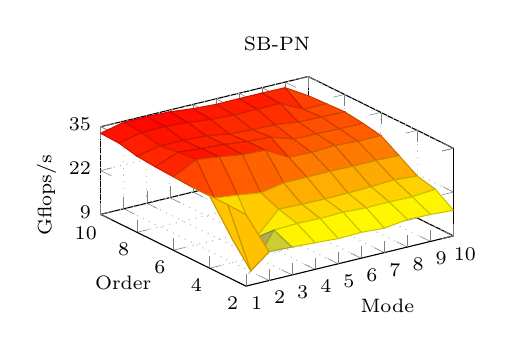
\begin{tikzpicture}
\begin{axis}[height=0.35\textwidth,width=0.5\textwidth,style={font=\scriptsize},grid=major,grid style={dotted},align=center,xlabel={Mode},ylabel={Order},zlabel={Gflops/s},title={\ttt{SB-PN}}, xtick={1,2,3,4,5,6,7,8,9,10},xticklabels={1,2,3,4,5,6,7,8,9,10}, ytick={2,4,6,8,10}, yticklabels={2,4,6,8,10}, point meta max=35, point meta min=9, zmin=9, zmax=35, ztick={9,22,35}, zticklabels={9,22,35}, view={-35}{45}, xlabel style={yshift=2mm}, ylabel style={yshift=4mm}, zlabel style={yshift=-1mm,xshift=-4mm}]
\addplot3[surf] % , colormap = {whiteblack}{color(0cm)=(white);color(0.4cm) = (darkgray)}
coordinates{
(1.000,2.000,30.244) (1.000,3.000,30.448) (1.000,4.000,30.513) (1.000,5.000,30.521) (1.000,6.000,30.805) (1.000,7.000,31.123) (1.000,8.000,31.582) (1.000,9.000,32.837) (1.000,10.000,33.056) 

(2.000,2.000,17.544) (2.000,3.000,9.230) (2.000,4.000,15.792) (2.000,5.000,25.482) (2.000,6.000,34.267) (2.000,7.000,33.761) (2.000,8.000,32.969) (2.000,9.000,34.257) (2.000,10.000,34.664) 

(3.000,2.000,17.291) (3.000,3.000,19.621) (3.000,4.000,14.674) (3.000,5.000,24.720) (3.000,6.000,33.420) (3.000,7.000,33.220) (3.000,8.000,32.935) (3.000,9.000,34.433) (3.000,10.000,34.713) 

(4.000,2.000,16.905) (4.000,3.000,19.948) (4.000,4.000,21.543) (4.000,5.000,23.741) (4.000,6.000,32.390) (4.000,7.000,32.790) (4.000,8.000,32.688) (4.000,9.000,33.939) (4.000,10.000,34.455) 

(5.000,2.000,16.491) (5.000,3.000,19.785) (5.000,4.000,21.325) (5.000,5.000,25.035) (5.000,6.000,32.072) (5.000,7.000,31.950) (5.000,8.000,31.519) (5.000,9.000,33.185) (5.000,10.000,33.743) 

(6.000,2.000,16.671) (6.000,3.000,19.953) (6.000,4.000,21.260) (6.000,5.000,25.077) (6.000,6.000,28.310) (6.000,7.000,31.655) (6.000,8.000,31.193) (6.000,9.000,32.836) (6.000,10.000,33.351) 

(7.000,2.000,16.269) (7.000,3.000,19.634) (7.000,4.000,21.358) (7.000,5.000,25.149) (7.000,6.000,28.067) (7.000,7.000,29.384) (7.000,8.000,30.938) (7.000,9.000,32.937) (7.000,10.000,33.399) 

(8.000,2.000,17.174) (8.000,3.000,19.698) (8.000,4.000,21.570) (8.000,5.000,25.007) (8.000,6.000,28.450) (8.000,7.000,29.241) (8.000,8.000,30.115) (8.000,9.000,32.937) (8.000,10.000,33.406) 

(9.000,2.000,16.998) (9.000,3.000,19.599) (9.000,4.000,21.975) (9.000,5.000,25.064) (9.000,6.000,28.078) (9.000,7.000,29.100) (9.000,8.000,29.960) (9.000,9.000,29.632) (9.000,10.000,33.336) 

(10.000,2.000,16.611) (10.000,3.000,20.174) (10.000,4.000,21.453) (10.000,5.000,24.861) (10.000,6.000,28.132) (10.000,7.000,29.142) (10.000,8.000,29.866) (10.000,9.000,29.588) (10.000,10.000,29.300) 

};\end{axis}
\end{tikzpicture}
\begin{comment}
\begin{tikzpicture}
\begin{axis}[height=0.40\textheight,width=0.40\textwidth,style={font=\footnotesize},grid=major,grid style={dotted},align=center,xlabel={Kontraktionsmodus},ylabel={Tensorstufe},title={TLib-SB-PB3},scaled ticks=false,zticklabel=\pgfmathprintnumber{\tick},zlabel={Durchsatz [Gflops/s]},view={-45}{45}, zlabel={Standardfehler [\%]}]
\addplot3[surf]
coordinates{(1.000,2.000,4.915) (1.000,3.000,2.617) (1.000,4.000,3.193) (1.000,5.000,4.037) (1.000,6.000,4.649) (1.000,7.000,4.045) (1.000,8.000,4.268) (1.000,9.000,1.298) (1.000,10.000,0.649) 

(2.000,2.000,1.146) (2.000,3.000,12.575) (2.000,4.000,10.226) (2.000,5.000,3.407) (2.000,6.000,1.272) (2.000,7.000,1.332) (2.000,8.000,1.219) (2.000,9.000,0.793) (2.000,10.000,0.947) 

(3.000,2.000,1.573) (3.000,3.000,1.382) (3.000,4.000,6.180) (3.000,5.000,3.661) (3.000,6.000,2.150) (3.000,7.000,1.692) (3.000,8.000,0.904) (3.000,9.000,0.674) (3.000,10.000,1.161) 

(4.000,2.000,2.256) (4.000,3.000,1.618) (4.000,4.000,1.501) (4.000,5.000,1.999) (4.000,6.000,1.755) (4.000,7.000,1.631) (4.000,8.000,1.231) (4.000,9.000,0.488) (4.000,10.000,0.991) 

(5.000,2.000,2.165) (5.000,3.000,1.481) (5.000,4.000,1.653) (5.000,5.000,2.982) (5.000,6.000,2.611) (5.000,7.000,2.199) (5.000,8.000,1.877) (5.000,9.000,0.945) (5.000,10.000,0.484) 

(6.000,2.000,1.881) (6.000,3.000,1.437) (6.000,4.000,1.837) (6.000,5.000,2.992) (6.000,6.000,2.179) (6.000,7.000,3.249) (6.000,8.000,2.066) (6.000,9.000,1.171) (6.000,10.000,0.683) 

(7.000,2.000,1.280) (7.000,3.000,1.511) (7.000,4.000,1.790) (7.000,5.000,2.757) (7.000,6.000,2.313) (7.000,7.000,2.193) (7.000,8.000,1.944) (7.000,9.000,1.215) (7.000,10.000,0.680) 

(8.000,2.000,2.513) (8.000,3.000,1.442) (8.000,4.000,1.953) (8.000,5.000,2.795) (8.000,6.000,2.272) (8.000,7.000,2.173) (8.000,8.000,1.382) (8.000,9.000,1.317) (8.000,10.000,0.759) 

(9.000,2.000,2.432) (9.000,3.000,1.826) (9.000,4.000,1.406) (9.000,5.000,2.650) (9.000,6.000,2.476) (9.000,7.000,2.317) (9.000,8.000,1.006) (9.000,9.000,1.365) (9.000,10.000,0.782) 

(10.000,2.000,2.422) (10.000,3.000,1.313) (10.000,4.000,2.697) (10.000,5.000,2.971) (10.000,6.000,2.301) (10.000,7.000,1.950) (10.000,8.000,1.294) (10.000,9.000,1.121) (10.000,10.000,0.678) 

};\end{axis}
\end{tikzpicture}
\end{comment}
